\section{Raycasting mittels front-to-back rendering}
\begin{figure}[H]
	\centering
	\begin{tikzpicture}[]
		\draw[rotate around={-45:(.5,1)}] (0,0) grid[step=.2] (1,2);
		\draw[-latex] (0,-1) -- (0,3);
		\draw (-1,-1) -- (3,-1) node[rotate=0, pos=.25] {\fbox{$~~$}};
		\foreach \j in {0,...,5} {
			\draw ($\j*(0,.25)+(0,.1)$) node [circle, fill=black, inner sep = 1pt] {};	
		}
		
		\draw (1,-1) node[rotate=0] {\fbox{$~~$}};
		\draw[-latex] (1,-1) -- (1,3);
		\foreach \j in {0,...,5} {
			\draw ($\j*(0,.25)+(1,.8)$) node [circle, fill=black, inner sep = 1pt] {};	
		}
	\end{tikzpicture}
\end{figure}
Auf der Sichtlinie werden in regelmäßigen Abständen im Körper Messpunkte gesetzt. Für jeden Messpunkt wird nun, wie vorher beschrieben, die Farbe und Leuchtkraft bestimmt. Anschließend werden diese zu einer Farbe für den entsprechenden Pixel auf dem Bildschirm zusammengefasst. Wir beginnen dabei mit dem entferntesten und enden mit dem Messpunkt am nähesten. Dadurch werden Voxel, welche hinter "`soliden"' Voxeln liegen in der Farbwahl nicht betrachtet.
\chapter{Einschub: Algebraische Flächen}
\[ f(x,y,z) = 0 \]
\[ \text{z.B.}~~\left\{ (x,y,z) \left| x^2 + y^2 + z^2  - 1 = 0 \right.  \right\} \]
\begin{figure}[H]
	\centering
	\begin{tikzpicture}
	\draw (.3,.8) circle (.5);
	\draw[rotate around={-45:(.5,1)}] (0,0) grid[step=.2] (1,2);
	\draw[-latex] (0,-1) -- (0,3);
	\draw (-1,-1) -- (3,-1) node[rotate=0, pos=.25] {\fbox{$~~$}};
	\foreach \j in {0,...,5} {
		\draw ($\j*(0,.25)+(0,.1)$) node [circle, fill=black, inner sep = 1pt] {};	
	}
	
	\draw (1,-1) node[rotate=0] {\fbox{$~~$}};
	\draw[-latex] (1,-1) -- (1,3);
	\foreach \j in {0,...,5} {
		\draw ($\j*(0,.25)+(1,.8)$) node [circle, fill=black, inner sep = 1pt] {};	
	}
	\end{tikzpicture}
\end{figure}

\begin{figure}[H]
	\centering
	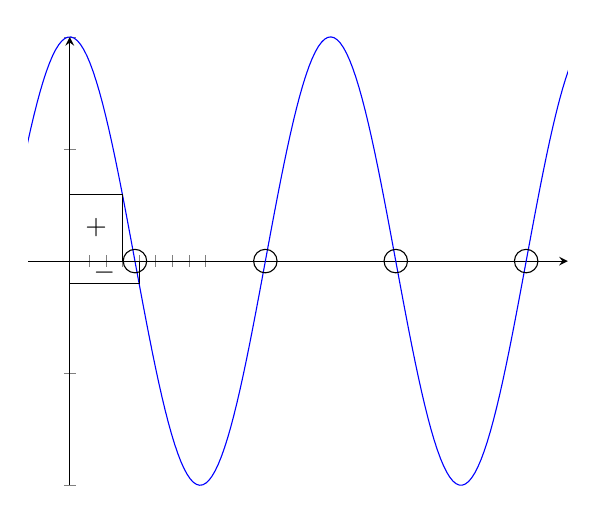
\begin{tikzpicture} % Ergänze makiere Nullpunkte, zeichne abtastrate auf x achse makiere letzte + und erst - stelle bei nullpunkt
	\begin{axis}[xmin = -1, xmax = 12 , yticklabels={,,}, xticklabels={,,}, axis lines = center, xtick={0.47,0.87,1.27,1.67,2.07,2.47,2.87,3.27}]
	\addplot[draw=blue, domain=-2:13, samples = 200] {cos(deg(x))};
	\draw (0,0) rectangle (1.27, {cos(deg(1.27))});
	\draw ({1.27/2}, {cos(deg(1.27))/2}) node {$+$};
	\draw (0,0) rectangle (1.67, {cos(deg(1.67))});
	\draw ({1.67/2}, {cos(deg(1.67))/2}) node {$-$};
	\draw ({pi/2}, 0) node[draw, circle, inner sep = 3] {};
	\draw ({pi/2+pi}, 0) node[draw, circle, inner sep = 3] {};
	\draw ({pi/2+2*pi}, 0) node[draw, circle, inner sep = 3] {};
	\draw ({pi/2+3*pi}, 0) node[draw, circle, inner sep = 3] {};
	\end{axis}
	\end{tikzpicture}
	\caption{Finden von Nullstellen durch Suche nach Vorzeichenwechsel}
\end{figure}
Wie beim Raycasting wird der Bereich in Abschnitte unterteilt und diese einzeln untersucht, folgt auf ein $+$ ein $-$ (oder umgekehrt), liegt dazwischen eine Nullstelle.
\[ p~~\nabla f(p) = n \]